%% Paul Johnson
%% 20180801

% standalone class for individual image to be included in a document
% border=15pt controls the whitespace padding around the diagram
\documentclass[border=15pt]{standalone}


\usepackage{tikz}

%% http://www.texample.net/tikz/examples/energy-level-diagram/
\usepackage[hang,small,bf]{caption}
\setlength{\captionmargin}{25pt}

\tikzset{
	% Two node styles for game trees: solid and hollow
	square node/.style={rectangle,draw,inner sep=1.5},
	middle node/.style={circle,draw=gray,dashed,inner sep=1.5},
    solid node/.style={circle,draw,inner sep=1.5, fill=black},
	hollow node/.style={circle, draw, inner sep=1.5}
}
\begin{document}

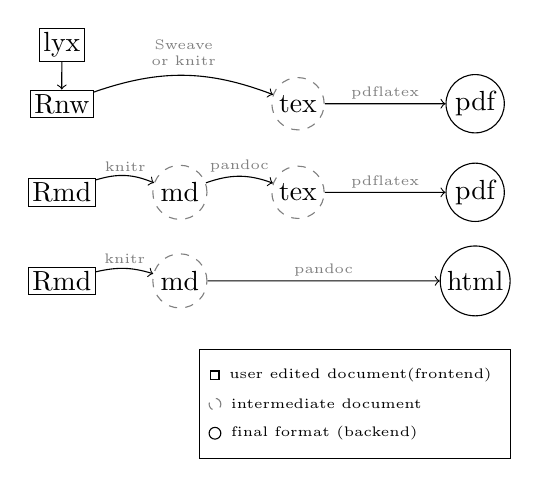
\begin{tikzpicture}[scale=1.5, font=\normalsize]

  \node(lyx) at (1, 0.75) [square node]{lyx} ;
  \node(rnw) at (1, 0.25) [square node]{Rnw};
  \node(tex) at (3, 0.25) [middle node]{tex};
  \node(pdf) at (4.5 , 0.25) [hollow node]{pdf};
  
  \path[->] (lyx) edge (rnw);
  \path[->] (rnw) edge [bend left=20] node[above, gray, very thin, text centered,
  text width=.5in, font=\tiny]{Sweave or knitr} (tex) ;
  \path[->] (tex) edge node[above, gray, very thin, text centered,
  text width=.5in, font=\tiny, inner sep=1.5]{pdflatex}(pdf);

  \node(rmd) at (1, -0.5) [square node]{Rmd};
  \node(md) at (2, -0.5) [middle node]{md};
  \node(tex) at (3, -0.5) [middle node]{tex};
  \node(pdf2) at (4.5, -0.5) [hollow node]{pdf}; 

  \path[->] (rmd) edge [bend left=20] node[above, gray, very thin, text centered,
  text width=.5in, font=\tiny, inner sep=1.5]{knitr} (md);
  \path[->] (md) edge [bend left=20] node[above, gray, very thin, text centered,
  text width=.5in, font=\tiny, inner sep=1.5]{pandoc}(tex);
  \path[->] (tex) edge node[above, gray, very thin, text centered,
  text width=.5in, font=\tiny, inner sep=1.5]{pdflatex}(pdf2);

  \node(rmd2) at (1, -1.25) [square node]{Rmd};
  \node(md2) at (2, -1.25) [middle node]{md};
  \node(html) at (4.5 , -1.25) [hollow node]{html}; 

  \path[->] (rmd2) edge [bend left=15] node[above, gray, very thin, text centered,
  text width=.5in, font=\tiny, inner sep=1.5]{knitr} (md2);
  \path[->] (md2) edge node[above, gray, very thin, text centered,
  text width=.5in, font=\tiny, inner sep=1.5]{pandoc}(html);

  %% insert empty node to create space between graph and legend
  \node(space) at (4.5, -1.75) []{};
  \matrix[draw, row sep=-\pgflinewidth, below left, font=\tiny] at (current bounding box.south east){
    \node [square node,label=right:user edited document(frontend)] {}; \\
    \node [middle node,label=right:intermediate document] {}; \\
    \node [hollow node,label=right:final format (backend)] {}; \\
  };
  
\end{tikzpicture}
\end{document}

  